\documentclass[11pt, xcolor={dvipsnames}, hyperref={colorlinks, allcolors=Blue}]{beamer}


% Packages
\usepackage{graphicx}
\usepackage{caption, subcaption}
\usepackage{tikz}
\usepackage{amsmath, amsfonts, amssymb}
\usepackage{bm}
\usepackage{booktabs}
\usepackage{apacite}
\usepackage{multirow}
\usepackage{doi}
\usepackage{textpos}
\usepackage{lipsum}
\usepackage{amsfonts, amsmath}
\usepackage{wrapfig}
\usepackage{animate}
\usepackage{cleveref}


\renewcommand\doiprefix{}


\usepackage{tikz}
\usetikzlibrary{shapes, fit}





%%%%%%%%%%%%%%%%%%%%%%%%%%%%%%%%%%%%%%%%%%%%%%
% Custom commands
\newcommand\bc[1]{{\usebeamercolor[fg]{frametitle} {\textbf{#1}}}} % bold and color
\newcommand{\into}{\rightarrow}



%%%%%%%%%%%%%%%%%%%%%%%%%%%%%%%%%%%%%%%%%%%%%%
% Set Theme
\usetheme{Boadilla}
\usecolortheme{rose}

%%%%%%%%%%%%%%%%%%%%%%%%%%%%%%%%%%%%%%%%%%%%%%
% Make citation font tiny
\renewcommand{\bibliographytypesize}{\tiny}

%%%%%%%%%%%%%%%%%%%%%%%%%%%%%%%%%%%%%%%%%%%%%%
% Fonts
\usefonttheme{serif} % Serif font
\setbeamertemplate{enumerate items}[default] % Don't use bullets in enumerate.

%%%%%%%%%%%%%%%%%%%%%%%%%%%%%%%%%%%%%%%%%%%%%%%
% Remove navigation bar
\setbeamertemplate{navigation symbols}{}
%%%%%%%%%%%%%%%%%%%%%%%%%%%%%%%%%%%%%%%%%%%%%%


% Frontmatter
\title[ECON 8000 -  Lecture 4]{Lecture 4: Linear Algebra II}
\author[University of Queensland]{Robert Garrard}
\date[\today]{} 


%%%%%%%%%%%%%%%%%%%%%%%%%%%%%%%

% Common commands

% Sets
\newcommand{\R}{\mathbb{R}}
\newcommand{\N}{\mathbb{N}}
\newcommand{\Z}{\mathbb{Z}}
\newcommand{\Q}{\mathbb{Q}}
\renewcommand{\P}{\mathbb{P}}
\newcommand{\E}{\mathbb{E}}

% Symbols
\renewcommand{\epsilon}{\varepsilon}
\renewcommand{\implies}{\Rightarrow}
\newcommand{\halmos}{\hfill$\blacksquare$}

% Vector notation
\renewcommand{\a}{\mathbf{a}}
\renewcommand{\b}{\mathbf{b}}
\newcommand{\x}{\mathbf{x}}
\newcommand{\X}{\mathbf{X}}
\newcommand{\y}{\mathbf{y}}
\newcommand{\z}{\mathbf{z}}
\renewcommand{\v}{\mathbf{v}}
\newcommand{\bepsilon}{\mathbf{\varepsilon}}
\newcommand{\bbeta}{\mathbf{\beta}}

% Matrices
\newcommand{\eyetwo}{\begin{pmatrix} 1 & 0\\ 0 & 1 \\ \end{pmatrix}} % I_2 identity matrix
\newcommand{\eyethree}{\begin{pmatrix} 1 & 0 & 0\\ 0 & 1 & 0\\ 0 & 0 & 1 \end{pmatrix}} % I_3 identity matrix
\newcommand{\zerotwo}{\begin{pmatrix} 0 & 0\\ 0 & 0 \\ \end{pmatrix}} % 2x2 Zero matrix
\newcommand{\zerothree}{\begin{pmatrix} 0 & 0 & 0\\ 0 & 0 & 0\\ 0 & 0 & 0 \end{pmatrix}} % 3x3 Zero matrix


% Misc

\newcommand{\innerprod}[2]{\langle #1, #2 \rangle}


%%%%%%%%%%%%%%%%%%%%%%%%%%%%%%%%

% Tikz
\usetikzlibrary{arrows,shapes,trees, positioning}

%%%%%%%%%%%%%%%%%%%%%%%%%%%%%%

\newcounter{Lecture}
\addtocounter{Lecture}{4}

\newcounter{exercise}
\newenvironment{exercise}[1][]{\refstepcounter{exercise}\par\medskip
   \noindent {\bc{Exercise}~\bc{\theLecture.\theexercise} #1}}{\medskip}


\begin{document}

\begin{frame}
\titlepage

%\begin{picture}(0,0)
%\put(35,-50){\hbox{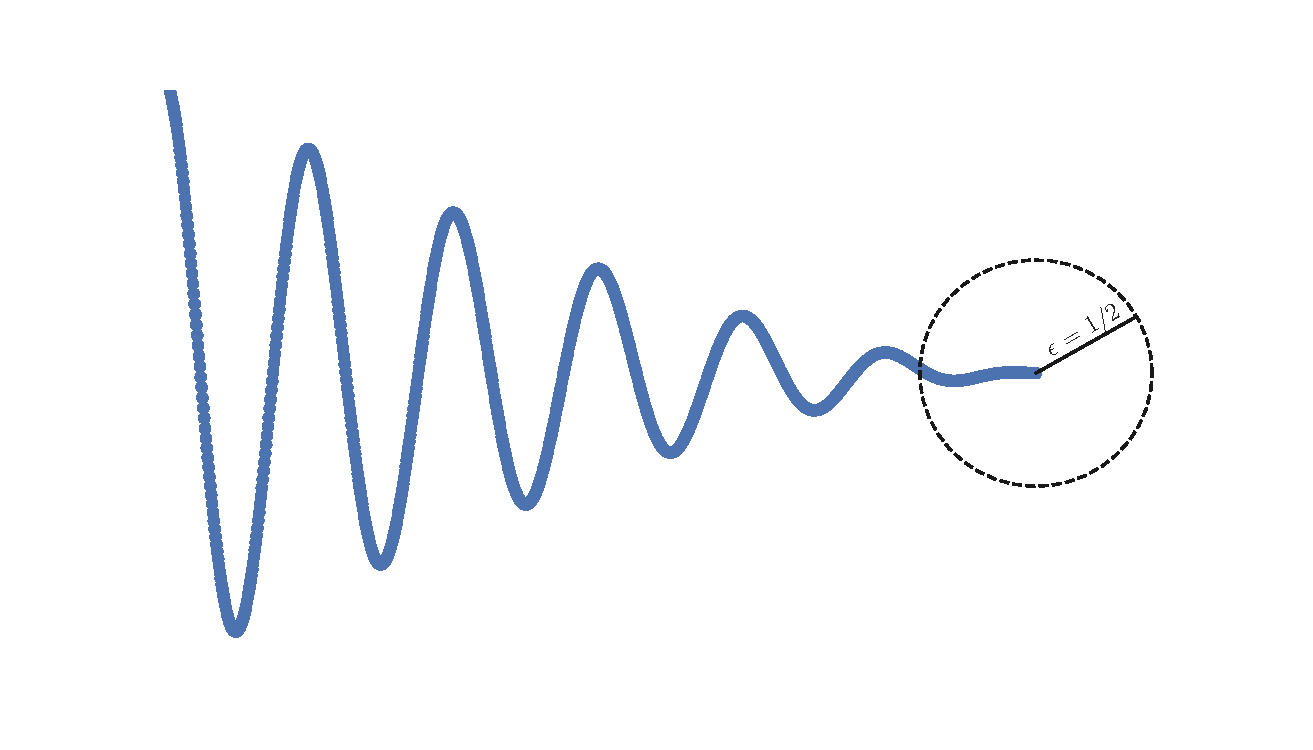
\includegraphics[width=0.8\textwidth, trim={0cm, 1cm, 0cm, 1cm}, clip]{convergence.pdf}}}
%\end{picture}

\end{frame}
%%%%%%%%%%%%%%%%%%%%%%%%%%%%%

\begin{frame}{Normed vector spaces}
Recall that the definition of a vector space allows us to perform the operations of ``addition'' and ``scalar multiplication'' on elements of the set. Note that the definition does not require a notion of ``distance'' or ``length''.\bigskip

A \bc{normed vector space} is a pair $(V, ||\cdot||)$ where $V$ is a vector space and $||\cdot||:V\rightarrow \R$ is a function with the following properties
\begin{enumerate}
\item $||\mathbf{0}|| = 0$  and  $||\x|| > 0$  if $\x \not = \mathbf{0}$

\item $||\alpha \x|| = |\alpha| \, ||\x||$  for any scalar $\alpha$

\item $||\x + \y|| \leq ||\x|| + ||\y|| \ \ \ \forall \x,\y \in V$
\end{enumerate}
\bigskip

\begin{exercise}
Show that $||x - y||$ is a metric.
\end{exercise}

\end{frame}

%%%%%%%%%%%%%%%%%%%%%%%%%%%%%
\begin{frame}{Normed vector spaces}

In Euclidean space, we'll most often use one of the $\ell_{p}$ norms ($p\geq 1$):

\[||\x||_{p} = \left( \sum_{i} |x_{i}|^{p} \right)^{\frac{1}{p}}\]
\bigskip

Usually one of the following particular cases:\medskip

\begin{itemize}
	\item The standard Euclidean norm: $||\x||_{2} = \sqrt{x_{1}^{2} + \dots + x_{n}^{2}}$

	\item The $\ell_1$ norm: $||\x||_{1} = \sum |x_{i}|$

	\item The sup-norm, or $\ell_\infty$ norm: $||\x||_{\infty} = \max\{| x_{1}|, \dots, |x_{n}|\}$
\end{itemize}
\end{frame}
%%%%%%%%%%%%%%%%%%%%%%%%%%%%%
\begin{frame}{Inner product spaces}
Norms endow a space with a notion of length, which induces a notion of distance between vectors. We can add an extra layer of structure to gain a notion of ``angle'' between two vectors.\bigskip

An \bc{inner product space} is a pair $(V, \innerprod{\cdot}{\cdot})$, where $V$ is a vector space and $\innerprod{\cdot}{\cdot}:V^{2}\to \R$, such that:

\begin{enumerate}
	\item $\innerprod{\v}{\v}\geq 0$ (Positivity)
	\item $\innerprod{\v}{\v} = 0$ iff $\v = 0$ (Definiteness)
	\item $\innerprod{\x}{\y} = \innerprod{\y}{\x}$ (Symmetry)
	\item $\innerprod{\x + \y}{\v} = \innerprod{\x}{\v} + \innerprod{\y}{\v}$ (Additivity)
	\item $\innerprod{\alpha \x}{\y} = \alpha \innerprod{\x}{\y}$ (Homogeneity)
\end{enumerate}

\end{frame}
%%%%%%%%%%%%%%%%%%%%%%%%%%%%

\begin{frame}{Euclidean Inner Product}
Let $\a = (a_{1},...,a_{n})$ and $\b = (b_{1},..., b_{n})$ be vectors in $\R^{n}$.  The \bc{Euclidean inner product} of $\a$ and $\b$ is the scalar
\[\a \cdot \b = a_{1}b_{1} + a_{2}b_{2} + ... + a_{n}b_{n}\]
\bigskip

\begin{exercise}
\begin{enumerate}
\item Show that the dot product is an inner product.
\item What norm is induced by the inner product?
\end{enumerate}
\end{exercise}

\end{frame}


%%%%%%%%%%%%%%%%%%%%%%%%%%%%%
\begin{frame}{Euclidean Inner Product}

\begin{theorem}
Let $\a$ and $\b$ be vectors in $\R^{n}$. Let $\theta$ be the angle between them. Then,
\[ \a \cdot \b = ||\a|| \, ||\b|| \, \cos{\theta}\]
\end{theorem}
 (This will come in handy when we talk about gradients)


\end{frame}
%%%%%%%%%%%%%%%%%%%%%%%%%%%%%
\begin{frame}{Matrix Algebra}
 Recall that matrices are $m\times n$ arrays of entries taken from a field (we'll only talk about the reals).\bigskip

Matrix addition is componentwise:

\[
\begin{pmatrix}
a_{1,1} & \dots & a_{1,n}\\
\vdots & a_{i,j} & \vdots\\
a_{m,1} & \dots & a_{m,n}
\end{pmatrix} 
+
\begin{pmatrix}
b_{1,1} & \dots & b_{1,n}\\
\vdots & b_{i,j} & \vdots\\
b_{m,1} & \dots & b_{m,n}
\end{pmatrix} 
\]

\[= 
\begin{pmatrix}
a_{1,1} + b_{1,1} & \dots & a_{1,n} + b_{1,n}\\
\vdots & a_{i,j}+b_{i,j} & \vdots\\
a_{m,1} + b_{m,1} & \dots & a_{m,n} + b_{m,n}
\end{pmatrix} 
\]
\end{frame}
%%%%%%%%%%%%%%%%%%%%%%%%%%%%%%%%%%%%%%%
\begin{frame}{Matrix Algebra}
as is scalar multiplication:\bigskip

\[
r
\begin{pmatrix}
a_{1,1} & \dots & a_{1,n}\\
\vdots & a_{i,j} & \vdots\\
a_{m,1} & \dots & a_{m,n}
\end{pmatrix} 
= 
\begin{pmatrix}
ra_{1,1} & \dots & ra_{1,n}\\
\vdots & ra_{i,j} & \vdots\\
ra_{m,1} & \dots & ra_{m,n}
\end{pmatrix} 
\]


\end{frame}
%%%%%%%%%%%%%%%%%%%%%%%%%%%%%%%%%%%%%%%

\begin{frame}{Matrix Algebra}
For two matrices, $A$ and $B$, we can define a new operation, matrix multiplication, in terms of inner products:

\[(AB)_{ij} = \a_{i} \cdot \b_{j}\]

where $\a_{i}$ and $\b_{j}$ are the $i$th row of $A$ and $j$th column of $B$ respectively.\bigskip

This is only well-defined if the matrices are \bc{conformable} to multiplication: the number of columns in the first matrix must equal the number of rows in the second.
\end{frame}

%%%%%%%%%%%%%%%%%%%%%%%%%%%%%%%%%%%%%%%

\begin{frame}{Matrix Algebra}
\begin{block}{Example}
\[
\underset{\hspace{-2mm} 3\times 2  \quad \quad \quad 2 \times 2}{
\begin{pmatrix}
a & b\\
c & d\\
e & f
\end{pmatrix}
\begin{pmatrix}
W & X\\
Y & Z
\end{pmatrix}
}
=
\underset{3\times 2}{
\begin{pmatrix}
aW + bY & aX + bZ\\
cW + dY & cX + dZ\\
eW + fY & eX + fZ
\end{pmatrix}
}
\]

Observe that the matrices conform to multiplication: $(3 \times \underbar{2}) \ \times \ (\underbar{2} \times 2) = 3 \times 2$\\

\end{block}
\end{frame}
%%%%%%%%%%%%%%%%%%%%%%%%%%%%%%%%%%%%%
\begin{frame}{Matrix Algebra}
We can \bc{transpose} an $m \times n$ matrix $A$, to form the $n\times m$ matrix $A^{\prime}$.\bigskip

When transposing a product, we reverse the order: $(ABC)^{\prime} = C^{\prime}B^{\prime}A^{\prime}$.\bigskip

Matrices that are their own transpose are called \bc{symmetric}: $A^{\prime} = A$.\bigskip

If $A$, $B$, and $C$ are invertible: $(ABC)^{-1} = C^{-1} B^{-1} A ^{-1}$.\bigskip

Matrices whose inverse is their transpose are called \bc{orthogonal}: $A^{-1} = A^{\prime}$.\bigskip

$(AB)^{-1^{\prime}} = (B^{\prime} A^{\prime})^{-1}$\bigskip

The \bc{trace} of a square matrix is the sum of its diagonal entries: $trace(A) = \sum_{i} A_{ii}$.

\end{frame}
%%%%%%%%%%%%%%%%%%%%%%%%%%%%%%%%%%%%%
%%%%%%%%%%%%%%%%%%%%%%%%%%%%%%%%%%%%%
\begin{frame}{Matrix Algebra}
\begin{exercise}
	\begin{enumerate}
		\item Let $A$ and $B$ be $n\times n$ matrices. Show that $trace(AB) = trace(BA)$.
		\item Show that $trace(A + B) = trace(A) + trace(B)$.
		\item Show that there are no square matrices with the property $AB - BA = I$.
	\end{enumerate}	
\end{exercise}
\end{frame}
%%%%%%%%%%%%%%%%%%%%%%%%%%%%%%%%%%%%%
\begin{frame}{Matrix Algebra}
If $A$ is an $m \times n$ matrix and $B$ is a $p\times q$ matrix, the \bc{kronecker product} of these two matrices is a block matrix of size $mp \times nq$ \bigskip


\[ A \otimes B =
\begin{pmatrix}
a_{1,1} B & \dots & a_{1,n} B\\
\vdots & \ddots & \vdots\\
a_{m,1} B & \dots & a_{m,n} B
\end{pmatrix}
\]
\bigskip

\end{frame}

\begin{frame}{Matrix Algebra}
\begin{block}{Example}
\[
A =
\begin{pmatrix}
1 & 2\\
3 & 4
\end{pmatrix}
\quad 
B = \eyetwo
\]

\[
A \otimes B = 
\begin{pmatrix}
1 \cdot \eyetwo & 2 \cdot \eyetwo\\
3 \cdot \eyetwo & 4 \cdot \eyetwo
\end{pmatrix}
\]

\[
=
\begin{pmatrix}
1 & 0 & 2 & 0\\
0 & 1 & 0 & 2\\
3 & 0 & 4 & 0\\
0 & 3 & 0 & 4
\end{pmatrix}
\] 
\end{block}

\end{frame}

%%%%%%%%%%%%%%%%%%%%%%%%%%%%%%%%%%%%%
\begin{frame}{Matrix Algebra}
The \bc{outer product} is a special case of the kronecker product where we're multiplying a column vector with a row vector.\bigskip



\[\a = 
\begin{bmatrix}
a_{1}\\
a_{2}\\
\vdots\\
a_{n}
\end{bmatrix}
\quad\quad
\b^{'} = 
\begin{bmatrix}
b_{1}, b_{2}, \dots, b_{n}
\end{bmatrix}
\]

\[
\a \b^{\prime} = 
\begin{bmatrix}
a_{1}b_{1} & a_{1}b_{2}&\dots& a_{1}b_{n}\\
\vdots & \cdots & \vdots & \vdots\\
a_{n} b_{1} & a_{n}b_{2} & \dots & a_{n}b_{n}
\end{bmatrix}
\]


\end{frame}
%%%%%%%%%%%%%%%%%%%%%%%%%%%%%%%%%%%%%
\begin{frame}{Matrix Algebra}

\begin{itemize}
\setlength{\itemsep}{5mm}
\item Conventionally, vectors are assumed to be column vectors.
\item When we want to write a row vector, we usually do it as the transpose of a column vector. 
\item A row vector times a column vector, $\a^{\prime} \b$, represents an \bc{inner product}
\item A column vector times a row vector, $\a \b^{\prime}$ represents an \bc{outer product}.
\end{itemize}

\end{frame}
%%%%%%%%%%%%%%%%%%%%%%%%%%%%%%%%%%%%%
\begin{frame}{Projection}
\begin{figure}[H]
\centering

\includegraphics[width=\textwidth]{mapprojection.jpg}
\end{figure} 

Projection involves ``pushing'' a vector from one space into a particular subspace.

\end{frame}

%%%%%%%%%%%%%%%%%%%%%%%%%%%%%%%%%%%%%
\begin{frame}{Projection}
A \bc{linear projection} is a square matrix $P$ that is idempotent. That is:\bigskip

\[P^{2} = P\]
\bigskip

Intuitively, this property means that once the matrix $P$ pushes a vector into a subspace, applying the projection again will just yield the same results. Anything which is already in the subspace stays where it is.


\end{frame}
%%%%%%%%%%%%%%%%%%%%%%%%%%%%%%%%%%%%%

\begin{frame}{Projection}

It's often the case that we wish to break a vector down into the sum of two vectors which are orthogonal.\bigskip

 That is, turn $\y$ into $\y = \hat{\y} + \mathbf{e}$ such that $\y^{\prime}\mathbf{e} = 0$. \bigskip

Moreover, we may want $\hat{\y}$ to lie in a particular subspace.

\end{frame}
%%%%%%%%%%%%%%%%%%%%%%%%%%%%%%%%%%%%%
\begin{frame}{Projection}

The \textbf{orthogonal projector} of a matrix $\X$ with full column rank is 
\[ \mathbf{P}_{\X} = \X\left(\X^{\prime}\X\right)^{-1}\X^{\prime}\]

\begin{exercise}
\begin{enumerate}
	\item Show that the orthogonal projector is in fact a projection.
	\item Show that $\mathbf{P}_{\X}$ is a symmetric matrix.
	\item Let the fitted value be $\hat{\y} = \mathbf{P}_{\X}\y$ and the residual, $\mathbf{e} = \y - \mathbf{P}_{\X}\y$. Show that $\hat{\y}^{\prime}\mathbf{e} = 0$.
	\item Show that $\X^{\prime}\mathbf{e} = 0$.
\end{enumerate}
\end{exercise}

\end{frame}

%%%%%%%%%%%%%%%%%%%%%%%%%%%%%%%%%%%%%
\begin{frame}{Approximate Solutions to Linear Equations}

Suppose we had a system of linear equations, $A\x = \y$, for which $A$ is an $n \times k$ matrix with full column rank and $n > k$.\bigskip

That is, there are more equations than unknowns, but the unknowns are linearly independent. \bigskip

Suppose further that the augmented system, $[A \ | \ \y]$ also has full rank. \bigskip

That is to say, two rows contain contradictory information.\bigskip

How many solutions are there to the system?\bigskip

Could we get an approximate solution to this system?
\end{frame}



\begin{frame}{Approximate Solutions to Linear Equations}
Let's pick some candidate solution $\x^{*}$.\bigskip


The error we make using $\x^{*}$ as our approximate solution is $\bepsilon = \y - A\x^{*}$.\bigskip

 A ``good'' solution should attempt to minimize this error.\bigskip

 Since this error is a vector, a reasonable choice might be to minimize the length of this vector, $|| \y - A\x^{*}||$.\bigskip

 Recall that (under the Euclidean norm) $||\bepsilon|| = \sqrt{\epsilon_1^2 + \cdots + \epsilon_n^2}$. Minimising the length of the vector is equivalent to minimising the sum of squared errors.
\end{frame}

%%%%%%%%%%%%%%%%%%%%%%%%%%%%%%%%%%%%

\begin{frame}{Approximate Solutions to Linear Equations}

So we have a vector $\y$ that is \emph{not} in the column space of $A$; otherwise there would be a solution.\medskip

 We're trying to find a vector in the column space of $A$ such that the distance between that vector and $\y$ is minimised.\medskip

 That is, we're trying to \emph{project} $\y$ into the column space of $A$.\medskip

 To be minimum distance, we specifically want to drop a \emph{perpendicular} from the tip of $\y$ into the col space of $A$.\medskip

 Recall that the shortest distance between a point and a line forms a right angle between the two.\medskip

 The same principle is operating here. As you may of guessed, we want the \emph{orthogonal projection} of $\y$ into the column space of $A$.
\end{frame}


\begin{frame}{Projection}
\begin{figure}[H]
\centering
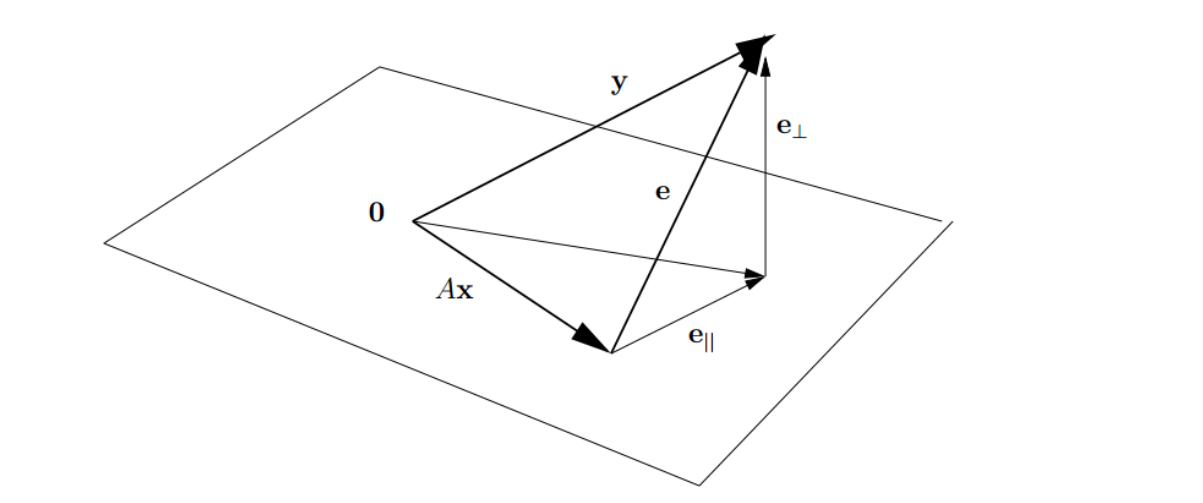
\includegraphics[width=\textwidth]{least_squares.png}
\caption{Orthogonal Projection}
\caption*{Source: http://www.math.ku.edu/~lerner/LAnotes/LAnotes.pdf}

\end{figure}
\end{frame}

%%%%%%%%%%%%%%%%%%%%%%%%%%%%%%%%%%%%

\begin{frame}{Economic Application: Ordinary Least Squares}
Let's say we wish to estimate the following multiple linear regression model.

\[ y_{i} = \beta_{0} + \beta_{1}x_{1,i} + \dots + \beta_{k}x_{p,i} + \epsilon_{i} \quad \quad i = 1,\dots,n\]

\bigskip
Why don't we make this more compact by stacking them in vectors and matrices?
\[ \y = \X \bbeta + \bepsilon\]
\medskip

Where $\y$ and $\bepsilon$ are $n\times 1$ vectors, $\X$ is an $n\times (p+1)$ matrix with $n > p+1$ and full column rank, and $\beta$ is a $(p+1)\times 1$ vector.
\end{frame}
%%%%%%%%%%%%%%%%%%%%%%%%%%%%%%%%%%%%

\begin{frame}{Economic Application: Ordinary Least Squares}
What is it we're asking for when we run an OLS regression?\bigskip

We're trying to find the causal effect of each $x$ variable on $y$; typically interpreted as ``if $x_1$ goes up by one unit, $y$ goes up $\beta_1$ units on average''. \bigskip

Another way to say this is that we're looking for a solution to the deterministic model $\y = \X \bbeta$. \bigskip

To solve this we need a $\bbeta$ in the column space of $\X$.\bigskip

The system typically has no solution (why?), so we need to approximate a solution by projecting $\y$ into the column space of $\X$. \bigskip

OLS picks $\bbeta$ to minimize the sum of square residuals. I.e., the projection of $\y$ into $\text{Col}(\X)$ must be an \emph{orthogonal} projection.
\end{frame}

\begin{frame}{Economic Application: Ordinary Least Squares}

\begin{exercise}
\begin{enumerate}
	\item Show that $\hat{\bbeta}_{OLS} = \left(\X^{\prime} \X\right)^{-1} \X^{\prime} \y$ solves the least squares problem.

	\item Show that $\hat{\bbeta}_{OLS}$ is unique.

	\item Suppose $\X$ is rank deficient. What is the solution set? How does it affect fitted values $\hat{\y}$?
\end{enumerate}
\end{exercise}
\end{frame}

%%%%%%%%%%%%%%%%%%%%%%%%%%%%%%%%%%%
\begin{frame}{Eigenvalues and Eigenvectors}
First let's recall that a matrix $A$ may be thought of as a linear map between two vector spaces. That is, it takes as input a vector $\x \in \R^m$ and transforms it into another vector, $A\x \in \R^n$.\bigskip


Let $A:\R^{n}\to\R^{n}$ be a linear map. An \bc{eigenvector} $\v$ of $A$ and its corresponding \bc{eigenvalue}, $\lambda$, are a vector and scalar satisfying 
\[ A\v = \lambda\v\]
\bigskip

\bc{Exercise:}
Why are eigenvectors only defined for square matrices? 
\end{frame}


\begin{frame}{Eigenvalues and Eigenvectors}
\begin{align*}
 &A\v = \lambda\v \\
 \Rightarrow \quad & \lambda\v - A\v  = 0\\ 
 \Rightarrow \quad &(\lambda\mathbf{I} - A)\v = 0
\end{align*}

But if $(\lambda\mathbf{I} - A)\v = 0$ for some non-zero vector $\v$, then $(\lambda\mathbf{I} - A)$ can't be full rank (why?).\bigskip

Since it's a square matrix, if it's not full rank then it must be singular! That is, it must be the case that

\[\det(\lambda \mathbf{I} - A) = 0\]

This determinant expands to an $n$th order polynomial in $\lambda$ called the \bc{characteristic equation}.
\end{frame}
%%%%%%%%%%%%%%%%%%%%%%%%%%%%%%%%%%%
\begin{frame}{Eigenvalues and Eigenvectors}

\begin{block}{Example}
\[ A = \begin{pmatrix} 0 & 1\\ -2 & -3\end{pmatrix} \]

Find the characteristic equation for $A$ and determine $A$'s eigenvalues.

\begin{align*}
 \det(\lambda \mathbf{I} - A) &= \left | \begin{pmatrix}\lambda & 0 \\ 0 & \lambda\end{pmatrix}   - \begin{pmatrix} 0 & 1\\ -2 & -3\end{pmatrix} \right |\\
\smallskip
&= \left | \begin{pmatrix}\lambda & -1 \\ 2 & \lambda + 3\end{pmatrix} \right |\\
\smallskip
&= \lambda(\lambda+3) - (-1)(2)\\
\smallskip
&= \lambda^{2} + 3\lambda +2
\end{align*}
Solving $\lambda^{2} +3\lambda +2 = 0$ yields $\lambda_1 = -1$, $\lambda_2 = -2$.
\end{block}
\end{frame}

\begin{frame}
Once we've obtained the set of eigenvalues, we can find their corresponding eigenvectors by solving the homogeneous system $(\lambda\mathbf{I}-A)\v = 0$ for $\v$. 

\begin{block}{Example (continued)}
First solve for $\lambda_1$. In order to solve $(-1\mathbf{I} - A)\v = 0$, simplify the term in brackets and construct an augmented system.
\begin{center}
\begin{tabular}{c  c c}
\begin{minipage}{0.2\textwidth}
\[
\left ( 
\begin{array}{c c | c}
-1 & -1 & 0\\ 2 & 2 & 0
\end{array} \right )
\]
\end{minipage}
\quad
\begin{minipage}{0.1\textwidth}
\[ \overset{rref}{\rightarrow}\]
\end{minipage}
\begin{minipage}{0.2\textwidth}
\[
\left ( 
\begin{array}{c c | c}
1 & 1 & 0\\ 0 & 0 & 0
\end{array} \right )
\]
\end{minipage}

\end{tabular}
\end{center}

Recall that to solve we set $x_2$ to be a free variable.

\begin{center}
\begin{minipage}{0.3\textwidth}
\begin{align*}
x_1 &= -x_2\\
x_2 &=x_2
\end{align*}
\end{minipage}
\quad 
\begin{minipage}{0.3\textwidth}
\[
\begin{pmatrix} x_1 \\ x_2 \end{pmatrix}
=
\begin{pmatrix} -1 \\ 1\end{pmatrix}x_2
\]
\end{minipage}
\end{center}
\end{block}
\end{frame}

%%%%%%%%%%%%%%%%%%%%%%%%%%%%%%%%%%%%
\begin{frame}{Eigenvalues and Eigenvectors}
\begin{block}{Example (continued)}
Doing the same for $\lambda_2$ gives
\begin{center}
\begin{tabular}{c  c c}
\begin{minipage}{0.2\textwidth}
\[
\left ( 
\begin{array}{c c | c}
-2 & -1 & 0\\ 2 & 1 & 0
\end{array} \right )
\]
\end{minipage}
\quad
\begin{minipage}{0.1\textwidth}
\[ \overset{rref}{\rightarrow}\]
\end{minipage}
\begin{minipage}{0.2\textwidth}
\[
\left ( 
\begin{array}{c c | c}
1 & \frac{1}{2} & 0\\ 0 & 0 & 0
\end{array} \right )
\]
\end{minipage}

\end{tabular}
\end{center}

Set $x_2$ to be a free variable.

\begin{center}
\begin{minipage}{0.3\textwidth}
\begin{align*}
x_1 &= -\frac{1}{2}x_2\\
x_2 &=x_2
\end{align*}
\end{minipage}
\quad 
\begin{minipage}{0.3\textwidth}
\[
\begin{pmatrix} x_1 \\ x_2 \end{pmatrix}
=
\begin{pmatrix} -\frac{1}{2} \\ 1\end{pmatrix}x_2
\]
\end{minipage}
\end{center}


Thus the eigenvector corresponding to $\lambda_1 = -1$ is $[-1, 1]^{\prime}$ and corresponding to $\lambda_2 = -2$ is $[-\frac{1}{2}, 1]^{\prime}$.
\end{block}


\end{frame}

%%%%%%%%%%%%%%%%%%%%%%%%%%%%%%%%%%%

\begin{frame}{Eigenvalues and Eigenvectors}

\begin{exercise}
\begin{enumerate}
	\item Verify manually that the above are actually eigenvectors.
	\item $[\frac{1}{2}, 1]^{\prime}$ is not very nice to look at. Is $[-1, 2]$ an eigenvector corresponding to $\lambda_2$? 
	\item Suppose $\v$ is an eigenvector of $A$. Is $k\v$ also an eigenvector for any scalar $k$? 
\end{enumerate}
\end{exercise}
\end{frame}
%%%%%%%%%%%%%%%%%%%%%%%%%%%%%%%%%%%

\begin{frame}{Diagonalization}
\begin{theorem}
Let $A$ be an $n\times n$ matrix. Let $\lambda_1,\dots,\lambda_n$ be eigenvalues of $A$ with corresponding eigenvectors $\v_1,\dots,\v_n$. Construct the matrix
\[P = [\v_1, \dots, \v_n]\]
whose columns are $A$'s eigenvectors. If $P$ in invertible, then
\[ P^{-1}AP = 
\left (
\begin{array}{c c c c }
\lambda_1 & 0 & \cdots & 0\\
0 & \lambda_2 & \cdots & 0\\
\vdots & \vdots & \cdots & \vdots\\
0 & 0 & 0 & \lambda_n
\end{array}
\right )
\]
\end{theorem}

\begin{exercise}
Verify that the matrix $A$ in the previous example is diagonalizable.
\end{exercise}

\end{frame}


%%%%%%%%%%%%%%%%%%%%%%%%%%%%%%%%%%%
\begin{frame}{Diagonalization}

But how do we know that the invertibility condition will be satisfied? We have a sufficient (but not necessary) condition!

\bigskip

\begin{theorem}
Let $\lambda_1,\dots,\lambda_n$ be $n$ \emph{distinct} eigenvalues of an $n\times n$ matrix. Then the corresponding eigenvectors are linearly independent.
\end{theorem}

\bigskip

If a matrix is not diagonalizable (called a \bc{defective} matrix), other methods may be available for solving the problem at hand (see Schur decomposotion).
\end{frame}
%%%%%%%%%%%%%%%%%%%%%%%%%%%%%%%%%%%
\begin{frame}{Diagonalization}
\begin{theorem}[The Spectral Theorem]
Let $A$ be an $n\times n$ matrix of real entries that is symmetric (i.e., $A^{\prime} = A$). Then $A$ can be diagonalized 

\[A = Q D Q^{\prime}\]

where $Q$ is an orthogonal matrix ($Q^{-1} = Q^{\prime}$).
\end{theorem}
\end{frame}
%%%%%%%%%%%%%%%%%%%%%%%%%%%%%%%%%%%
\begin{frame}{Systems of Difference Equations}
\[ x_{t+1} = a x_{t}\]

Perhaps $x_t$ is a bank balance and $a = 1+ r$ is the gross rate of return, for example. The solution to this is fairly straight forward and can be achieved through back substitution:

\[x_t = a^t x_0\]


An alternative way to say this is that 
\[x_t = c a^t\]
where $c$ is a constant determined by the boundary condition (initial value).

\end{frame}

%%%%%%%%%%%%%%%%%%%%%%%%%%%%%%%%%%%
\begin{frame}{Systems of Difference Equations}
But what about an arbitrary \emph{system} of first order linear difference equations. 

\begin{center}
\begin{tabular}{c c c c c c c c c}
$x_{1, t+1}$ & = & $a_{11}x_{1,t}$   &+&   $a_{12}x_{2,t}$      &+&    $\cdots$    &+&    $a_{1n}x_{n,t}$   \\
$x_{2, t+1}$ & = &$a_{21}x_{1,t}$   &+&   $a_{22}x_{2,t}$      &+ &   $\cdots$    &+&    $a_{2n}x_{n,t}$  \\
$x_{3, t+1}$ & = &$a_{31}x_{1,t}$   &+&   $a_{32}x_{2,t}$      &+&    $\cdots$    &+&    $a_{3n}x_{n,t}$ \\
$\vdots$ & =& $\vdots$               &+&        $\vdots$                &+&    $\cdots$    &+&    $\vdots$\\
$x_{n, t+1}$ & = & $a_{n1}x_{1,t}$  &+&   $a_{m2}x_{2,t}$   &+&    $\cdots$    &+&    $a_{nn}x_{n,t}$ 
\end{tabular}
\end{center}

Written more compactly as
\[ \x_{t+1} = A \x_{t}\]

\end{frame}

%%%%%%%%%%%%%%%%%%%%%%%%%%%%%%%%%%%
\begin{frame}{Systems of Difference Equations}

Suppose that A is diagonalizable. Such that we can right
\[A = PDP^{-1}\]

 We can consider the transformed system
 \begin{align*}
 \x_{t+1} &= A\x_t\\
 P^{-1}\x_{t+1} &= D\left ( P^{-1} \x_t\right)\\
 \z_{t+1} &= D \z_t
 \end{align*}


Such that $\x_t = P \z_t$ and $D$ is a diagonal matrix of the eigenvalues of $A$. 

\end{frame}

%%%%%%%%%%%%%%%%%%%%%%%%%%%%%%%%%%%
\begin{frame}{Systems of Difference Equations}

Can we solve this diagonal system? Actually, it's very easy. The diagonal matrix makes this system \bc{decoupled}. That is, each difference equation only depends on its own lag, not the lag of the other variables. That is
\begin{align*}
z_{1, t+1} &= \lambda_1 z_{1, t}\\
z_{2, t+1} &= \lambda_2 z_{2,t}\\
& \ \vdots\\
z_{n, t+1} &= \lambda_n z_{n, t}
\end{align*}

But we've seen how to easily solve these separate difference equations! 

\end{frame}

%%%%%%%%%%%%%%%%%%%%%%%%%%%%%%%%%%%
\begin{frame}{Systems of Difference Equations}

\begin{align*}
\begin{pmatrix} z_{1,t} \\ \vdots \\ z_{n,t} \end{pmatrix}
=
\begin{pmatrix} c_1 \lambda_1^t \\ \vdots \\ c_n \lambda_n^t\end{pmatrix}
\end{align*}

But we don't wish to know the solution in terms of $\z_t$, we want it in terms of $\x_t$. But recall that $\x_t = P\z_t$! Yielding

\begin{align*}
\x_t &= P\z_t\\
&= [\v_1, \dots, \v_n] \z_t\\
&= z_{1,t} \v_1 + \dots z_{n,t} \v_n\\
&= c_1 \lambda_1^t \v_1 + \dots + c_n \lambda_n^t \v_n
\end{align*}

The solution to a system of difference equations can be written as a linear combination of its eigenvectors!

\end{frame}

%%%%%%%%%%%%%%%%%%%%%%%%%%%%%%%%%%%
\begin{frame}{Quadratic Forms}

After linear functions, the next simplest are the \bc{quadratic forms}. 

A quadratic form on $\R^{n}$ is a real-valued function of the form\bigskip

\[\mathcal{Q}(x_{1},x_{2},\dots, x_{n}) = \sum_{i \leq j} a_{ij}x_{i}x_{j}\]
\bigskip

Any quadratic form can be written more compactly as
\bigskip

\[\mathcal{Q}(x_{1},\dots,x_{n}) = \x^{'}A\x\]
\bigskip

where $A$ is a unique real-valued symmetric matrix.

\end{frame}

%%%%%%%%%%%%%%%%%%%%%%%%%%%%%%%%%%%
\begin{frame}{Definiteness}
\begin{figure}
	\centering
	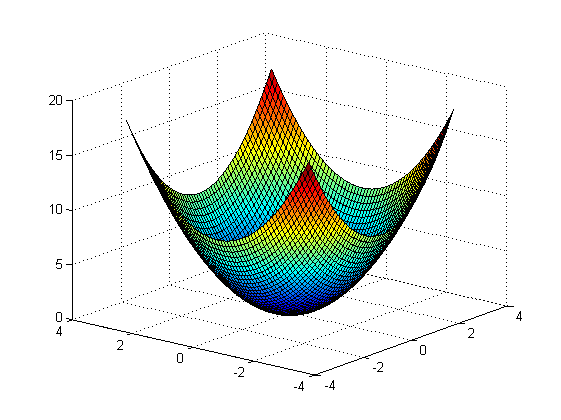
\includegraphics[width=0.75\textwidth]{quadraticform1.png}
	\caption{Positive Definite: $\mathbf{x}^{\prime}A\mathbf{x} > 0$}
\end{figure}
\end{frame}
%%%%%%%%%%%%%%%%%%%%%%%%%%%%%%%%%%%
\begin{frame}{Definiteness}
\begin{figure}
	\centering
	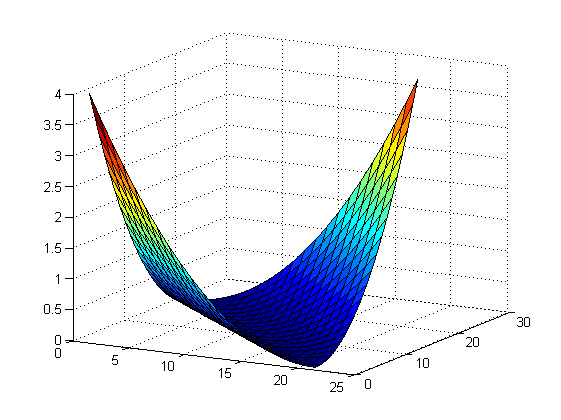
\includegraphics[width=0.75\textwidth]{quadraticform4.png}
	\caption{Positive Semi-definite: $\mathbf{x}^{\prime}A\mathbf{x} \geq 0$}
\end{figure}
\end{frame}

%%%%%%%%%%%%%%%%%%%%%%%%%%%%%%%%%%%
\begin{frame}{Definiteness}
\begin{figure}
	\centering
	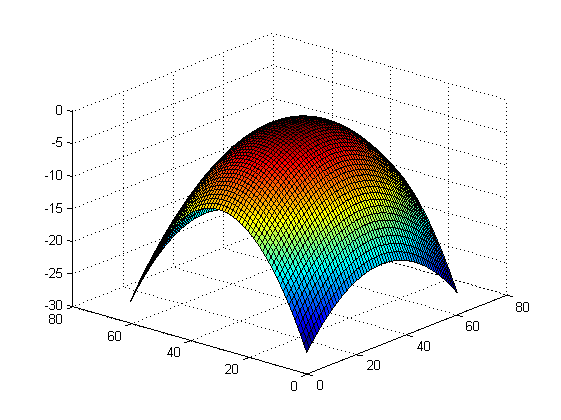
\includegraphics[width=0.75\textwidth]{quadraticform2.png}
	\caption{Negative Definite: $\mathbf{x}^{\prime}A\mathbf{x} < 0$}
\end{figure}
\end{frame}

%%%%%%%%%%%%%%%%%%%%%%%%%%%%%%%%%%%
\begin{frame}{Definiteness}
\begin{figure}
	\centering
	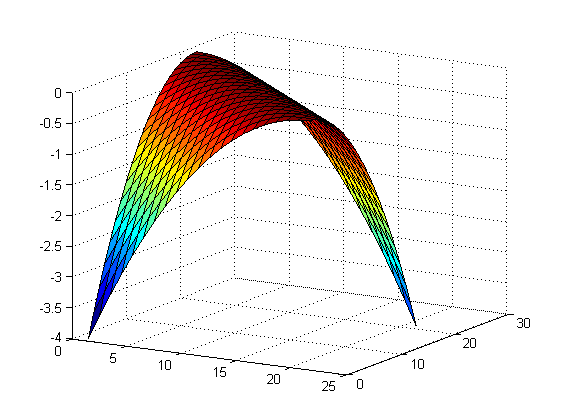
\includegraphics[width=0.75\textwidth]{quadraticform5.png}
	\caption{Negative Semi-definite: $\mathbf{x}^{\prime}A\mathbf{x} \leq 0$}
\end{figure}
\end{frame}

%%%%%%%%%%%%%%%%%%%%%%%%%%%%%%%%%%%
\begin{frame}{Definiteness}
\begin{figure}
	\centering
	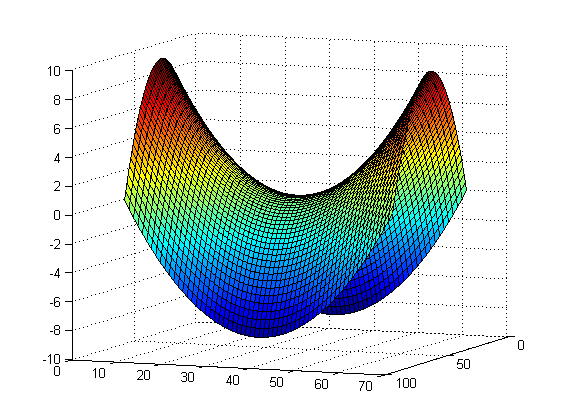
\includegraphics[width=0.75\textwidth]{quadraticform3.png}
	\caption{Indefinite: $\mathbf{x}^{\prime}A\mathbf{x} > 0$ for some $\mathbf{x}$, $\mathbf{x}^{\prime}A\mathbf{x} < 0$ for others.}
\end{figure}
\end{frame}

%%%%%%%%%%%%%%%%%%%%%%%%%%%%%%%%%%%
\begin{frame}{Definiteness}
\begin{theorem}
Let $A$ be a symmetric matrix. Then
\begin{enumerate}[a)]
\item $A$ is positive definite iff all eigenvalues are $> 0$.
\item $A$ is negative definite iff all eigenvalues are $< 0$.
\item $A$ is positive semidefinite iff all eigenvalues are $\geq 0$.
\item $A$ is negative semidefinite iff all eigenvalues are $\leq 0$
\item $A$ is indefinite iff it has at least one positive and one negative eigenvalue.  

\end{enumerate}
\end{theorem}

\end{frame}

%%%%%%%%%%%%%%%%%%%%%%%%%%%%%%%%%%%
\begin{frame}{Cholesky Decomposition}
\begin{theorem}[Cholesky Decomposition]
If $A$ is symmetric and positive definite, then $A$ can be decomposed as

\[A = C C^{\prime}\]

where $C$ is a lower-triangular matrix.
\end{theorem}
\end{frame}

%%%%%%%%%%%%%%%%%%%%%%%%%%%%%%%%%%%
\begin{frame}{Learning Outcomes}

\bc{You should be able to:}
\begin{itemize}
	\item Show that a function is a valid norm or inner product.
	\item  Perform common matrix operations.
	\item Construct the orthogonal projector for a matrix.
	\item Find the eigenvalues and eigenvectors of a matrix.
	\item Diagonalize a matrix.
	\item Solve very simple linear dynamical systems.
	\item Determine the definiteness of a square matrix.
\end{itemize}


\end{frame}


\end{document}